\newcommand{\ClassPath}{../../VIU_TFM_LaTeX_template}
\documentclass{\ClassPath/viu-tfm-template}
\usepackage{multicol}

\definecolor{maincolor}{HTML}{f25416}

%--------------------------------------------------------------------------
% Definiciones necesarias Modifica con tus datos
%--------------------------------------------------------------------------
\def\nombre{Gómez Olivencia, Rubén}
\def\dni{78910013-A}
\def\titulo{Biblioteca de series en PHP}
\def\titulacion{Máster Universitario en Desarrollo de Aplicaciones y Servicios Web}
\def\curso{2022-2023}

%Los siguientes son opcionales: si no se ponen, la portada cambia un poco. Ideal para escribir artículos/trabajos cortos
\def\dirige{}
\def\convocatoria{}
\def\asignatura{Desarrollo de aplicaciones web I: Lado del servidor (\textit{back-end})}


% importar fichero de Bibliografía
%\addbibresource{Actividad_1.bib}

\begin{document}
\graphicspath{{../../VIU_TFM_LaTeX_template/}}

\coverpage

\tableofcontents

\chapter{Introducción}

A lo largo de este documento se van a explicar las decisiones tomadas, tanto en el ámbito de programación como de diseño, durante el desarrollo de una aplicación web para gestionar una biblioteca que contiene series, junto con los episodios y actores que contiene.

Para la realización de esta web se ha hecho uso del lenguaje de programación \href{https://www.php.net/}{PHP} para la parte \textit{\textbf{back-end}}, junto con \textbf{javascript} para la programación \textbf{\textit{front-end}}.


\chapter{Arquitectura cliente-servidor}
A la hora de realizar una aplicación web tenemos que tener en cuenta cómo funciona la arquitectura que hace posible que podamos interactuar con ella.

Cuando navegamos por internet se hace uso de la conocida como arquitectura \textbf{Cliente - Servidor}, en la que podemos diferenciar, como su nombre indica, dos apartados:

\vspace{-1em}
\begin{itemize}
    \item \textbf{Servidor}: Un servidor es un ordenador potente que recibe peticiones, las procesa y devuelve una respuesta dependiendo de la petición recibida. En el caso de una aplicación web, el servidor contará con un servicio que recibirá peticiones \textbf{HTTP} y responderá con respuestas en código HTML, imágenes, ficheros ... Entre los servidores web más conocidos están: \href{https://httpd.apache.org/}{Apache HTTP Server}, \href{https://nginx.org/}{Nginx}, \href{https://www.iis.net/}{IIS}, ...

    \item \textbf{Cliente}: A la hora de interactuar con una aplicación web el cliente es quien va a realizar las peticiones al servidor. Normalmente el cliente es un navegador web utilizado por un usuario. Entre los navegadores web más conocidos están: \href{https://www.mozilla.org/es-ES/firefox/}{Firefox}, \href{https://www.google.com/chrome/}{Chrome}, \href{https://www.microsoft.com/es-es/edge}{Edge}, ...
\end{itemize}
\vspace{-1em}

\section{Back-end vs. Front-end}
En la arquitectura explicada previamente, a la hora de diseñar el software, entran en juego también dos partes, que se encargarán por separado de procesar la entrada y realizar una salida:

\vspace{-1em}
\begin{itemize}
    \item El \textbf{\textit{back-end}} es el software que se ejecuta en la parte de \textbf{servidor}, que recibe las peticiones del cliente, las procesa (gestión de autenticación, acceder a base de datos, realizar cálculos, obtener información...) y que posteriormente el servidor devolverá.

    En este apartado de \textbf{\textit{back-end}} se hace uso de lenguajes de programación como \href{https://www.php.net/}{PHP} o \href{https://www.java.com/es/}{Java}, frameworks como \href{https://laravel.com/}{Laravel}, \href{https://rubyonrails.org/}{Ruby on Rails}... , por poner sólo unos ejemplos.

    \item El \textbf{\textit{front-end}} es la parte que se ejecuta en la parte \textbf{cliente} (navegador web) de la arquitectura anterior. Mostrará la información atendiendo al diseño recibido, teniendo en cuenta la información HTML y las hojas de estilos CSS.
\end{itemize}
\vspace{-1em}

La web creada ha sido realizada desde el punto de vista del desarrollo \textbf{\textit{back-end}}, programada enteramente en \textbf{PHP}, para, de esta manera, gestionar los eventos en el lado servidor, procesar los datos y devolverlos para ser mostrados en el navegador web.


\chapter{Requisitos del proyecto}

Como todo proyecto, existen unos requisitos que deben ser cumplidos al terminar el desarrollo. De manera resumida, los requisitos son los siguientes:

\vspace{-1em}
\begin{itemize}
    \item Biblioteca de series con 5 tablas (plataforms de emisión, series, actores, directores, idiomas y series).
    \item Uso del patrón \textbf{MVC} (Modelo - Vista - Controlador) a la hora     de programar.
    \item Al menos tres vistas para cada entidad
\end{itemize}
\vspace{-1em}

Como se verá a continuación, todos los requisitos se han cumplimentando, tras realizar una pequeña modificación al modelo de datos.

\chapter{Modelo de datos}
A la hora de gestionar una biblioteca de series, hay que tener en cuenta que estas cuentan con episodios, por lo que se ha añadido esta nueva entidad.

Por otro lado, dado que actor y director pueden ser el mismo, y aparte, puede haber mucha más gente involucrada en una serie, por lo tanto se ha decidido unificar dichas entidades en una, para después gestionar el papel que realizan por cada episodio.

El esquema \textbf{Entidad - Relación} final queda de la siguiente forma:

\begin{center}
    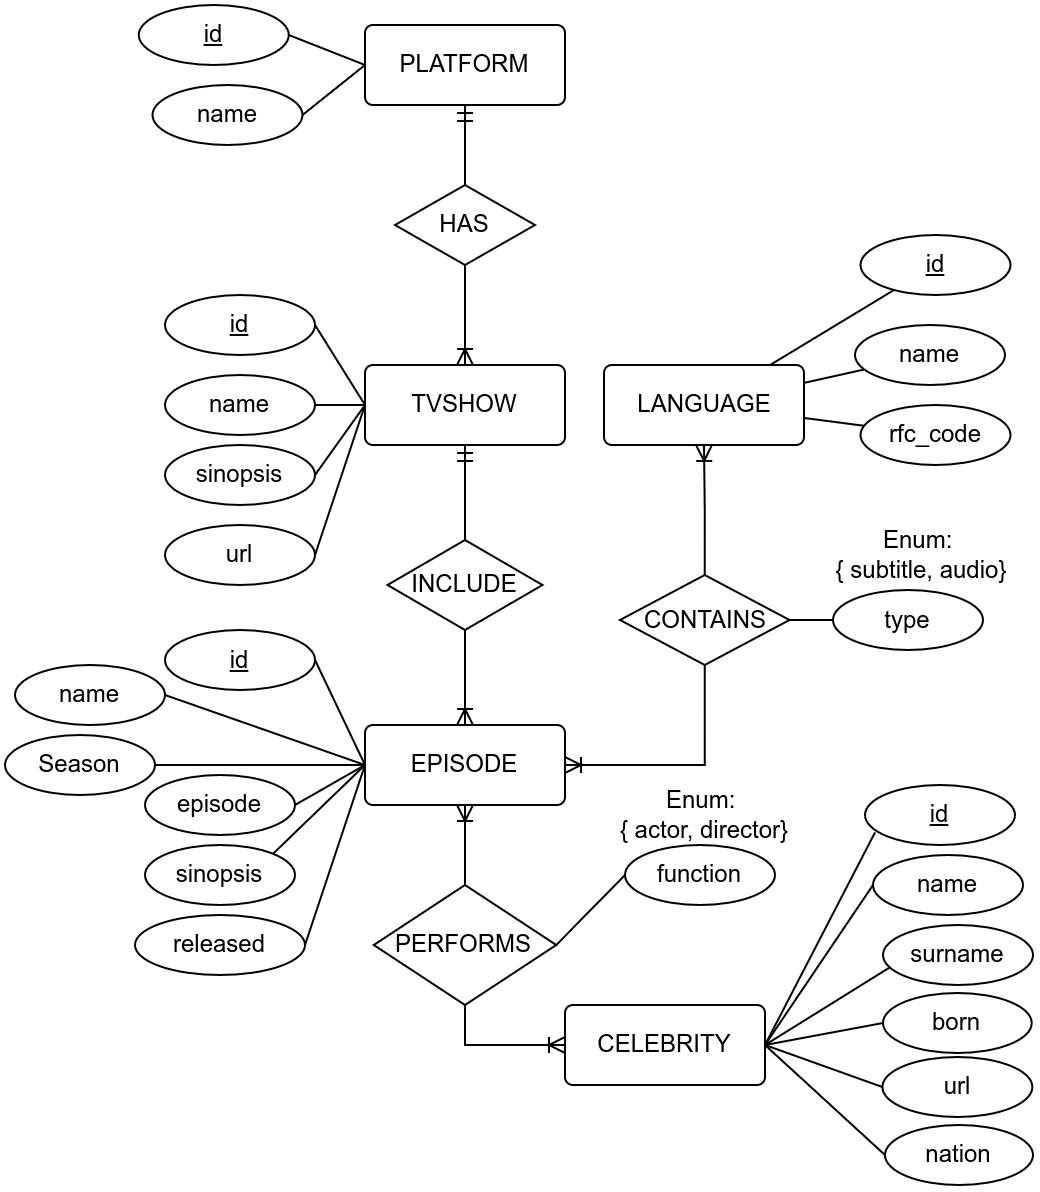
\includegraphics[width=0.8\linewidth]{img/entidad-relacion.png}
\end{center}


Este esquema entidad-relación ha dado lugar a un total de siete tablas cuyo esquema físico se puede importar desde el fichero \configfile{create_schema.sql} a MySQL, tal como veremos más adelante.

\chapter{Despliegue de la aplicación}
Antes de entrar en detalle en cómo se ha desarrollado la aplicación es importante conocer cómo podemos realizar el despliegue de la aplicación, ya sea para utilizarla o para realizaro modificaciones sobre la misma.

\section{Servicios Docker}
Para realizar el desarrollo del proyecto se ha utilizado servicios a través de contenedores \textbf{\href{https://www.docker.com/}{Docker}}, los cuáles pueden ser levantados gracias al fichero \configfile{compose.yaml} y el comando \commandbox{docker-compose up}
.


\begin{mycode}{Parte del fichero \textbf{compose.yaml}}{yaml}{}
services:
    php:
        image: docker.io/webdevops/php-nginx-dev:8.1
        ports:
            - '80:80'
        environment:
            - PHP_DISPLAY_ERRORS=1
            - PHP_DATE_TIMEZONE="Europe/Madrid"
        volumes:
            - './src:/app'
        depends_on:
            - mysql
\end{mycode}

Este fichero se encarga de desplegar los siguientes \textit{containers}:
\vspace{-1em}
\begin{enumerate}
    \item \textbf{PHP+Nginx}: Servicio de backend con el servidor web
    \href{https://nginx.org/}{Nginx} y el servicio \textbf{PHP FPM} para realizar el procesado de PHP.
    \item \textbf{MySQL}: Servidor de base de datos relacional donde irán los datos.
    \item \textbf{PHPMyAdmin}: Para gestionar de manera más sencilla la base de datos.
\end{enumerate}
\vspace{-1em}

Al levantar los servicios con el comando \textbf{docker-compose up} se hará uso de los siguientes puertos:
\vspace{-1em}
\begin{itemize}
    \item \textbf{80}: Para el entorno web.
    \item \textbf{3306}: Para la base de datos.
    \item \textbf{3307}: Para phpmyadmin.
\end{itemize}
\vspace{-1em}

\section{Despliegue del código fuente}
Para realizar el despliegue del código fuente sobre el contenedor de \textbf{PHP}, el directorio \configdir{src} debe estar situado a la misma altura del fichero \configfile{compose.yaml}.

De esta manera, a la hora de levantar el servicio se crea un volumen compartiendo el directorio local “src” con otro dentro del contenedor, en la ruta \configdir{/app}, que es de donde se nutre Nginx.


\section{Creación de la base de datos}

El servicio de MySQL se encarga de crear una base de datos llamada \textbf{actividad1} en el momento en el que el servicio se levanta. También crea los siguientes credenciales:

\vspace{-1em}
\begin{itemize}
    \item usuario:  \textbf{actividad1}
    \item contraseña:  \textbf{4ct1v1d4d1}
\end{itemize}
\vspace{-1em}

\section{Despliegue de datos}
Para realizar el despliegue de datos, vamos a hacer uso de los siguientes ficheros que acompañan esta memoria y el código fuente:

\vspace{-1em}
\begin{itemize}
    \item \textbf{create\_schema.sql}: Para realizar la creación de las tablas necesarias para el proyecto.
    \item \textbf{inserts.sql}: Para poblar las tablas con datos reales que pueden ser utilizados junto con la aplicación.
\end{itemize}
\vspace{-1em}

Estos ficheros se pueden importar a través del servicio \textbf{PHPMyAdmin} comentado previamente, a través del puerto 3307.


\chapter{Desarrollo realizado}

Una vez tenemos realizado el despliegue, se va a profundizar en el desarrollo realizado, destacando los siguientes aspectos:

\section{Configuración de la aplicación}
Aunque la aplicación realizada es sencilla, para evitar tener que estar repitiendo código, y buscando facilitar una futuro expansión del proyecto, se ha creado un fichero de configuración \configfile{config.php}.

Este fichero actualmente cuenta con una variable \inlineconsole{$conf}

\section{Modelo MVC}
Uno de los requisitos era hacer uso del modelo Modelo-Vista-Controlador (\textbf{MVC}), a la hora de programar. Es por ello que dentro del directorio entregado con el código fuente existen tres directorios principales dedicados a este modelo de programación:

\vspace{-1em}
\begin{itemize}
    \item \textbf{models}: Dentro de este directorio se encuentran los distintos modelos de datos que se utilizan dentro de la aplicación web. Estos modelos son creados a través de clases en PHP, que generan objetos. Debido al modelo relacional creado, algunas de las clases contienen como atributos otros objetos.

    Por ejemplo, un episodio tiene como atributo (a través de un identificador propio) la serie a la que pertenece, realizando de esta manera programación orientada a objetos, y a través de un episodio poder acceder a su elemento padre.

    \item \textbf{controllers}: En este directorio se encuentran distintos ficheros, uno por cada modelo existente, que contienen distintas funciones para ser el nexo de unión entre los modelos de datos y las vistas. En este directorio se quieren destacar dos ficheros “especiales”:
    \begin{itemize}
        \item \textbf{DB.php}: Este fichero contiene funciones que tienen que ver con la base de datos. Principalmente la gestión de la conexión a MySQL y el uso de una función genérica que recibe una query, la ejecuta y devuelve los valores. De esta manera se ha tratado de buscar la eficiencia y el no repetir código fuente a lo largo de la aplicación.

        \item \textbf{helpers.php}: Este es un fichero que contiene distintas funciones que pueden ser utilizadas a lo largo de toda la aplicación, y que no tienen que ver con un modelo concreto de datos.

        La creación de este fichero se ha basado en el \textit{framework} \textbf{Ruby On Rails}, el cual cuenta con unos ficheros “\_helpers.rb” cuya función es igual, la \textbf{no duplicación de código fuente}.
    \end{itemize}

    \item \textbf{views}: Directorio que contiene las vistas creadas para cada uno de los modelos, separados por directorios. En el siguiente punto se va a detallar más sobre este aspecto
\end{itemize}

\section{Creación de “plantillas” para las vistas}
Dado que en la aplicación web existe la posibilidad de mostrar información relacionada desde distintos apartados, se ha tratado de evitar la duplicación de cógido en la medida de lo posible creando un sistema de “plantillas” propio.

Vamos a poner un ejemplo sencillo, la \textbf{creación y edición de una celebrity}. Para crearla, se mostrará un  formulario con una serie de campos (nombre, apellido, fecha de nacicimento, ...) que deben ser rellenados antes de guardar la información.

A la hora de editar, se necesita un formulario que muestre la información para que pueda ser modificada. Es por eso, que en lugar de crear dos formularios en dos ficheros distintos, se ha creado un fichero \configfile{_form.php} que contiene el formulario propiamente y es importado desde los ficheros \configfile{new.php} y \configfile{edit.php}

Este uso de plantillas no sólo se ha limitado a los formularios, ya que también se ha utilizado para ciertos listados que muestran objetos:
\begin{center}
    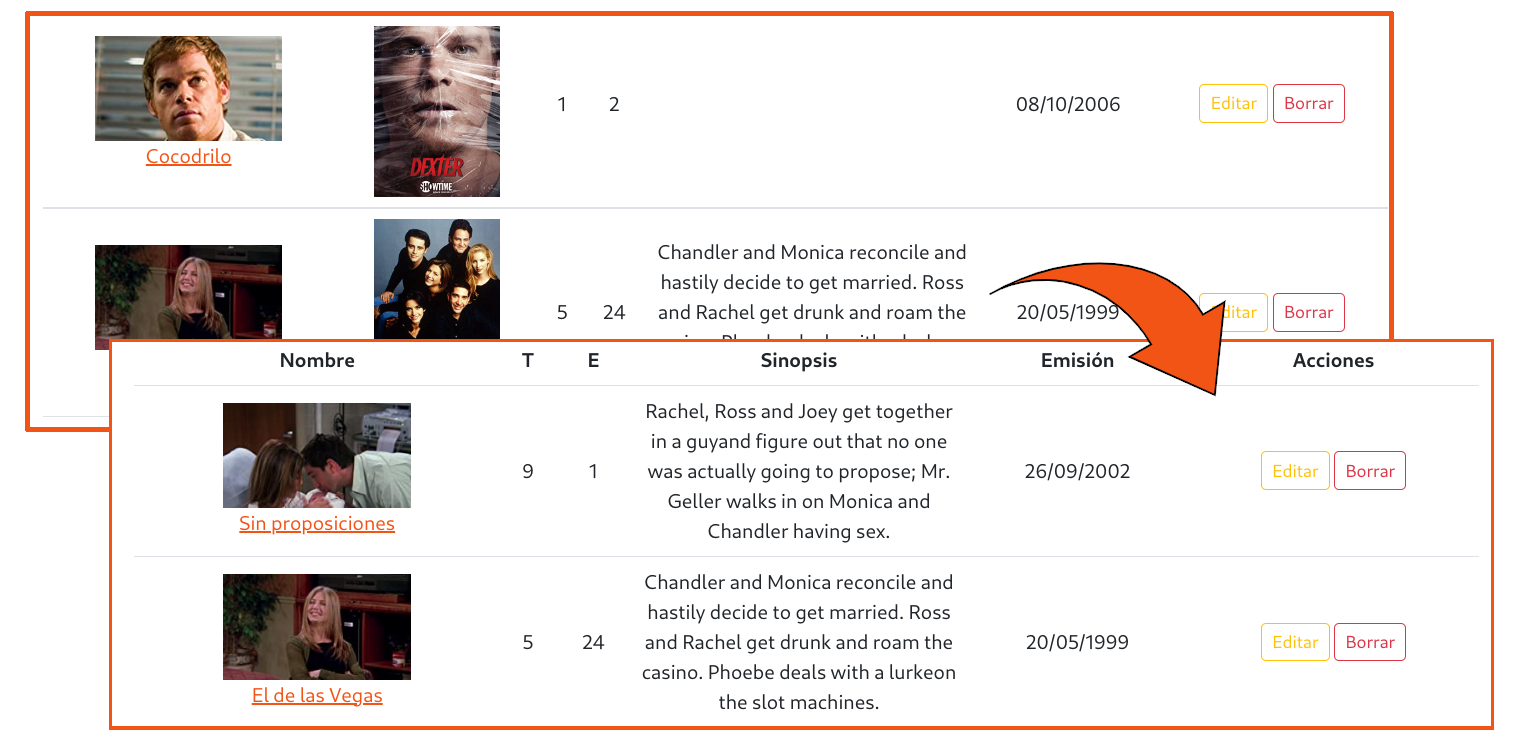
\includegraphics[width=0.8\linewidth]{img/vistas.png}
\end{center}

Tal como se puede ver en la imagen, existen dos listados que muestran episodios de series, pero que se visualizan en distintos sitios de la aplicación web (el listado general de episodios, y al ver una serie concreta).

Este ejemplo muestra los episodios de la serie “Friends” (a través de \href{http://localhost/views/tvshows/show.php?id=4}{este enlace}), que utiliza como fichero de plantilla  el \configfile{views/episodes/_list.php} que es incluído a través de la sentencia \inlineconsole{include_once("../episodes/_list.php");} desde la vista \configfile{views/tvshows/show.php}.

En algunos casos, como en el de la imagen, en la vista existe cierta programación para que teniendo en cuenta cuál es el origen, se muestren más columnas o menos.

Este sistema de plantillas es habitual en todo tipo de frameworks, que permiten aislar de mejor manera distintas secciones, e incluso permiten el paso de parámetros. En este caso se ha realizado de manera “más artesanal”, pero consiguiendo la finalidad, que es la no duplicidad de código.


\section{Uso de javascript para llamadas asíncronas}



\chapter{Aspecto visual}
Para mejorar el aspecto visual se ha hecho uso de la




\chapter{Dificultades del proyecto}

Como todo proyecto de programación, durante el desarrollo nos podemos encontrar con ciertas dificultades que deben ser subsanadas para llegar a cumplir los requisitos planteados al comienzo del proyecto.

% TODO: AÑADIR COSAS


\chapter{Conclusiones}

A la hora de afrontar un proyecto, es importante conocer las ventajas e inconvenientes que representa el lenguaje de programación que vamos a utilizar, así cómo el entorno de trabajo y los requisitos que se nos exige para afrontar el proyecto.

Este desarrollo ha permitido recordar las funcionalidades que los \textit{frameworks} nos permiten realizar de manera sencilla. De no poder contar con ellos, hay que tener en cuenta distintos aspectos para asegurar que la aplicación sea funcional y segura, para que el usuario pueda disfrutar de lo realizado, mientras que a la vez en caso de posibles ataques (inyección de código malicioso, XSS, ...) no se vea afectado ni el propio código, ni la base de datos.


%\printbibliography[title={Referencias bibliográficas},heading=bibintoc]

\end{document}
